\documentclass[a4 paper, 12pt]{article}
\usepackage{graphicx}
\usepackage{amssymb}
\usepackage{vmargin}
\usepackage{csquotes}
\usepackage{hyperref}
\usepackage{caption}
\setmargins{2.5cm}{1.5cm}{16.5cm}{23.42cm}{10pt}{1cm}{0pt}{2cm}
\graphicspath{ {.} }


\begin{document}
\title{Informe de la Tarea Investigativa II, presentado por los estudiantes del equipo No. 29}
\author{Anabel Ben\'itez Gonz\'alez C211 \\[10pt] Karen Dianelis Cantero L\'opez C211}

\date{15/12/2022}
\maketitle

\begin{center}
\large{T\'itulo: Fister-Panetta Upper Bound for Cancer Growth. Some 
Computational Remarks \\[10pt]}
\end{center}

Autores del art\'iculo:
\begin{itemize}
\item R\^{a}zvan Bocu
\item Dr Sabin Tabirca
\item Yin Jie Chen
\end{itemize}

\begin{center}
Publicado en : junio de 2008
\end{center}
\begin{center}
Conferencia Internacional de Biocomputaci\'on, Bioinform\'atica, y Tecnolog\'ias Biom\'edica, 2008.
\end{center}
 
\section{Valoraci\'on del Art\'iculo}
\subsection{Explicaci\'on de que trata}
Este art\'iculo resalta lo beneficioso que ser\'ia para la investigaci\'on del c\'ancer, una \mbox{cooperaci\'on} entre la biolog\'ia y las matem\'aticas. Primeramente se explica brevemente el c\'ancer en t\'erminos biol\'ogicos 
sencillos. Luego el art\'iculo presenta una descripci\'on de los modelos matem\'aticos y biocomputacionales actuales de la terapia y progresi\'on del c\'ancer. Explica la importancia de la modelaci\'on matem\'atica y 
la computaci\'on en la investigaci\'on del c\'ancer, argumentando que estas proveen a los investigadores herramientas que les permiten realizar experimentos computacionales que ser\'ian muy dif\'iciles de recrear en un ambiente 
experimental real, \mbox{entre} estos experimentos se encuentran modelar la evoluci\'on en el tiempo de estrategias de tratamiento ya usadas o incluso simular nuevas estrategias. Finalmente se propone una forma de optimizar la
administraci\'on del tratatamiento, basada en el modelo de Fister y Panetta, el cual es modificado en pos de mejorar sus predicciones.\\[10pt]

\subsection{Problem\'atica que se propone resolver}
El art\'iculo tiene como objetivo analizar el proceso de administraci\'on de la medicaci\'on contra el c\'ancer y proponer un modelo matem\'atico de optimizaci\'on para la administraci\'on del f\'armaco bas\'andose en
el estudio de la relaci\'on entre el medicamento y la oncog\'enesis (evoluci\'on del c\'ancer).

\subsection{T\'ecnicas utilizadas}
En el art\'iculo utilizan el modelo de Fister y Panetta, cuya ecuaci\'on analizaremos en la pr\'oxima secci\'on.

\subsection{Ecuaciones que ilustran el modelo matem\'atico usado}

Este modelo se representa en una sola ecuaci\'on:\\[10pt]
$\frac{dN}{dt} = rN(t)F(N) - G(N,u(t))$
donde N representa el volumen del tumor, r denota la tasa de crecimiento del tumor y F es una funci\'on que se relaciona con la evouci\'on de $\Theta$, que representa el tama\~{n}o m\'aximo del tumor. 
La funci\'on G describe la interacci\'on entre el tratamiento u(t) y el volumen del tumor N, debido a que la naturaleza de esta interacc\'on no est\'a bien definida, Fister y Panetta consideraron tres posibles relaciones:
\begin{enumerate}
\item La mayor\'ia de las c\'elulas cancer\'igenas mueren cuando el tumor alcanza su mayor volumen
\item El tratamiento es m\'as efectivo cuando el tumor es peque\~{n}o pero tiene la mayor tasa de crecimiento (basado en la enfermedad o linfoma de Hodgkin)
\item El tratamiento es menos efectivo cuando menor cantidad de prote\'inas est\'an disponibles para interactuar
\end{enumerate}

Se supone que la funci\'on F sigue la ley de crecimiento de Gompertzian: \\
$ F(N) = ln(\frac{\Theta }{N})$ \\[10pt]

Como ya mencionamos, la funci\'on $G(N, t)$ describe los efectos farmacocin\'eticos y farmacodin\'amicos del f\'armaco sobre el sistema. En su estudio, Fister y Panetta comparan tres estrategias para matar c\'elulas:  

\begin{itemize}
\item $G(N) = \delta u(t)N$: hip\'otesis de Skipper
\item $G(N) = \delta u(t)\frac{N}{K+N}$:  modelo de $E_{max}$  
\item $G(N) = \delta u(t)F(N)$: hip\'otesis de Norton–Simon
\end{itemize}


En estas ecuaciones $\delta$ es la magnitud de la dosis,  $u(t)$ describe la efectividad del f\'armaco dependiente del tiempo y K representa la afinidad del receptor por el fármaco. \\
Teniendo en cuenta las tres estrategias, y luego de escalar los modelos, se llega a lo conocido como : "L\'imite Superior de Fister-Panetta":

\begin{center}
$ P_{1} :  \frac{dN}{dt} = rNln(\frac{1}{N}) - u(t)\delta N$ \\[10pt]
$ P_{2}:  \frac{dN}{dt} = rNln(\frac{1}{N}) - u(t) \frac{\delta N}{k + N}$ \\[10pt]
$ P_{3}:  \frac{dN}{dt} = rNln(\frac{1}{N}) [1 - \delta u(t)]$

\end{center}

\subsection{Condiciones iniciales o de frontera}
Se considera que $G(N,t) = 0$ cuando no se usa ning\'un tratamiento efectivo. Se denota de forma simb\'olica $N(0) = N_{0}$ \\

\subsection{Resultados a los que arriban}
\begin{itemize}
\item Al resolver $P_{1}$, se obtiene que: $N(t) = (e^{e^C})^{e^{-rt+r\delta \int_0^t u(x)dx }}$. Teniendo el cuenta el caso cuando $t=0$, se obtiene como condici\'on incial que: $N(0) = e^{e^C} = N_{0}$ \\
Entonces se puede concluir $N(t) = (N_0)^{e^{-rt+r\delta \int_0^t u(x)dx }}$ 
\item $P_2$ no se pudo resolver por m\'etodos algebraicos.
\item Al resolver $P_{3}$ se obtiene que $N(t) = e^{\int_0^t{r \ln \frac{1}{x}(1-\delta u(x))dx}}$
\end{itemize}
Se concluye que$ \frac{dN}{dt} = rNln(\frac{1}{N}) $ representa una cota superior para el crecimiento del tumor, y $ P_{3}$ se acerca bastante a esta cota \\[10pt]
Al usar m\'etodos num\'ericos en las 3 ecuaciones y manteniendo las constantes : $u = 1, \delta = 0.1 ,$ y $r= [0.1, 0.05, 0.2]$ se obtienen los siguientes gr\'aficos: \ref{aprox}


Las gr\'aficas de $P_1$ y $P_2$  aparentan tener una tasa de crecimiento sensiblemente menos abrupta. En otras palabras, estos modelos matem\'aticos de la terapia de administraci\'on de medicamentos configuran las mejores opciones para diseñar una estrategia de administraci\'on de medicamentos y, por lo tanto, tienen m\'as posibilidades de ser utilizados para la calibraci\'on de la actividad m\'edica real.

\section{Ejemplos Num\'ericos}
\subsection{Puntos de Equilibrio y Estabilidad de Dichos Puntos}
Debido a que nuestro paper no contaba con un Sistema de Ecuaciones Diferenciales Ordinarias; usamos el sistema mostrado en el paper 31 [3] para realizar el an\'alisis de puntos de equilibrio y estabilidad de estos puntos.

\begin{center}
  $\displaystyle  \left\{
    \begin{array}{ll}
      x' = 4 \sqrt{3}r^{2}x + xy(x-4r) - \sqrt{3}rx^{2}\\
     y' = 0.5x^{2}y - 2rxy + y^{2}(\sqrt{3}r - 0.5y)
    \end{array}
\right.$
\end{center}

De este sistema de ecuaciones se han encontrado 6 puntos fijos
\begin{itemize}
\item $ P_{1} (0,0)$
\item $ P_{2} (0,2\sqrt{3}r)$
\item $ P_{3} (4r,0) $
\item $ P_{4} (4r,2\sqrt{3}r)$
\item $ P_{5} (r,\sqrt{3}r)$
\item $ P_{6} (r,\sqrt{3}r)$
\end{itemize}

La matriz Jacobiana del sistema es la siguiente:
\begin{displaymath}
  J =    \left(
      \begin{array}{cc}
        4 \sqrt{3}r^{2}-4ry +2xy - 2\sqrt{3}rx  & -4rx + x^2  \\
       xy - 2ry & 0.5x^2 -2rx + 2\sqrt{3}ry - 1.5y^2
      \end{array}
    \right)
\end{displaymath}

Analicemos el punto de equilibrio $ P_{2} (0,2\sqrt{3}r)$

La matriz Jacobiana en este punto quedar\'ia:

\begin{displaymath}
  J_{(0,2\sqrt{3}r)} =    \left(
      \begin{array}{cc}
        - 4 \sqrt{3}r^{2}  & 0  \\
      - 4 \sqrt{3}r^{2} & -6r^2
      \end{array}
    \right)
\end{displaymath}

De aqu\'i, la traza: $\tau = - 4 \sqrt{3}r^{2} -6r^2$, el determinante es : $\Delta = 24 \sqrt{3}r^4$ .\\[10pt]
Luego, $\tau ^2 - 4\Delta =  r^4(84 - 48 \sqrt{3}) $ \\[10pt]
Se cumple que : \\[10pt]
-$\Delta > 0$\\[10pt]
- $\tau ^2 - 4\Delta > 0$ \\[10pt]
- $\tau < 0 $ \\[10pt]
Entonces el punto $(0,2 \sqrt{3}r)$ representa un nodo estable. Su plano de fase se puede observar aqu\'i: \ref{plano}

\section{Conclusiones}
Este trabajo nos acerca a la investigaci\'on, muy fomentada en nuestra facultad. Gracias a esta asignatura contamos con las bases para poder adentrarnos en l\'ineas de investigac\'on muy importantes en la 
actualidad, algunas de las cuales pueden salvar la vida de miles e incluso millones de personas, con el uso de ecuaciones diferenciales se puede predecir y modelar la evoluci\'on de enfermedades y epidemias 
con bastante precisi\'on. El paper que analizamos en esta tarea, se enfoca mucho en algo que consideramos de suma importancia, la necesidad de colaboraci\'on entre bi\'ologos y matem\'aticos para lograr continuar 
avanzando en la investigaci\'on de una enfermedad tan problem\'atica para la sociedad contempor\'anea como lo es el c\'ancer. Relacionado a continuar en esta l\'inea de investigaci\'on, consideramos que nos 
faltan algunos conocimientos b\'asicos de biolog\'ia necesarios para entender las investigaciones previas del tema, este problema es f\'acil de solucionar dedicando algo de tiempo a su estudio, m\'as a\'un 
si se cuenta con un profesional que nos guie y ayude, por tanto estamos abiertas a la posibilidad de colaborar en investigaciones relacionadas con el c\'ancer y aportar nuestro granito de arena a la comunidad
cient\'ifica.

\section{Bibliograf\'ia Consultada}
\begin{enumerate}
\item C. Henry Edwards, Penney D.E., Calvis D. T. “Ecuaciones Diferenciales y Problemas con Valores en la Frontera”. Pearson Education, 2009.
\item Răzvan Bocu, Dr Sabin Tabirca, Yin Jie Chen. Fister-Panetta Upper Bound for Cancer Growth. Some Computational Remarks.
\item Joanna M. Chrobak, Henar Herrero. Un modelo matem\'atico de competici\'on entre c\'ancer y sistema inmune.
\end{enumerate}

\section{Anexos}
\begin{center}

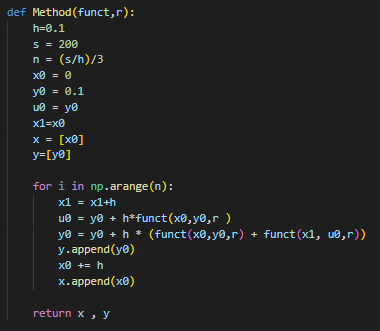
\includegraphics[width=0.5\textwidth]{EulerMej}
\captionof{figure} {M\'etodo de Euler Mejorado} \label{MetodoEuler}

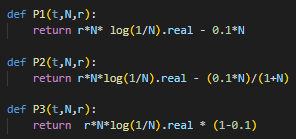
\includegraphics[width=0.5\textwidth]{func}
\captionof{figure} {Funciones $P_1 , P_2, P_3$} \label{Funciones $P_1 , P_2, P_3$}

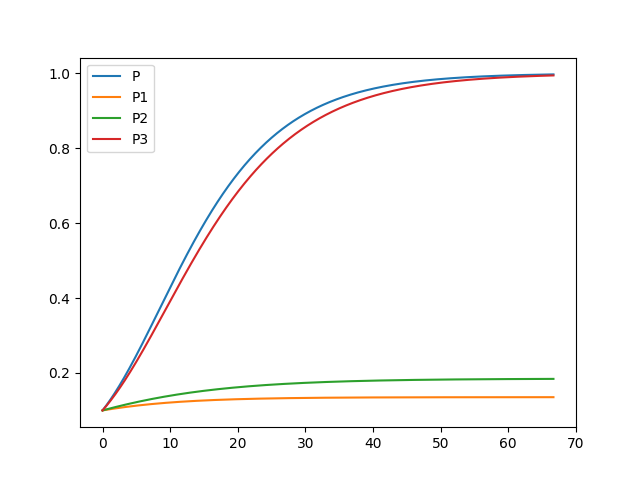
\includegraphics[width=0.5\textwidth]{r=0.05}
\captionof{figure} {Aproximaciones para r=0.05} \label{aprox}

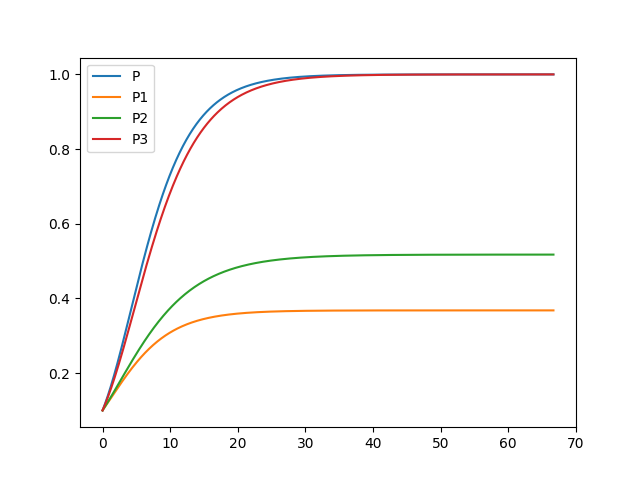
\includegraphics[width=0.5\textwidth]{r=0.1}
\captionof{figure} {Aproximaciones para r=0.1} \label{aprox1}

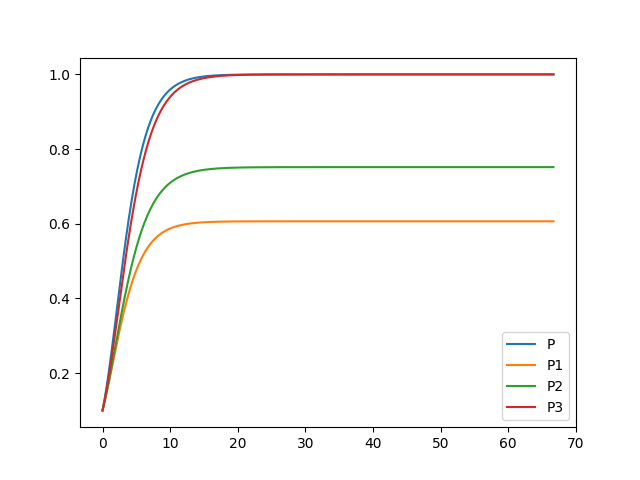
\includegraphics[width=0.5\textwidth]{r=0.2}
\captionof{figure} {Aproximaciones para r=0.2} \label{aprox2}

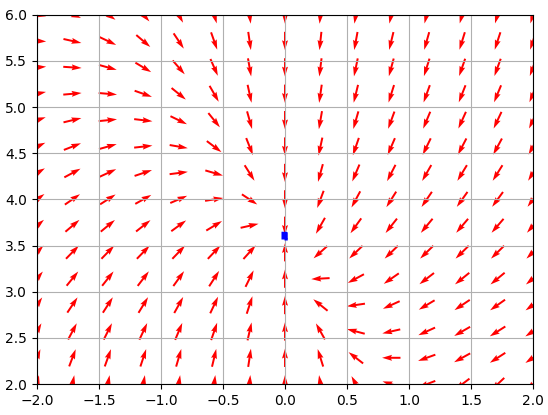
\includegraphics[width=0.8\textwidth]{fase lamba1}
\captionof{figure} {Plano de fases para r=1} \label{plano}

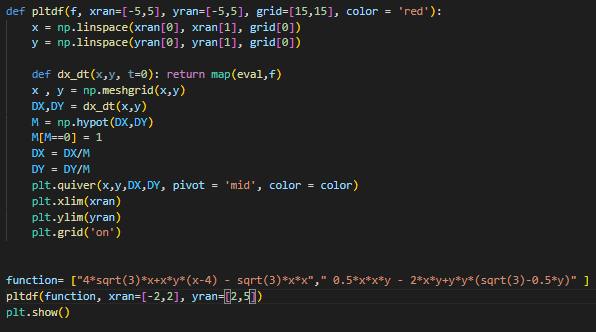
\includegraphics[width=0.8\textwidth]{codigofase}
\captionof{figure} {C\'odigo en python para generar el plano de fases} \label{codigofase}
\end{center}

\end{document}